\documentclass[border=5pt]{standalone}
\usepackage[T1]{fontenc}
\usepackage{lmodern}
\usepackage{pgfplots}
\usepgfplotslibrary{groupplots}
\pgfplotsset{compat=1.18}
\begin{document}\sffamily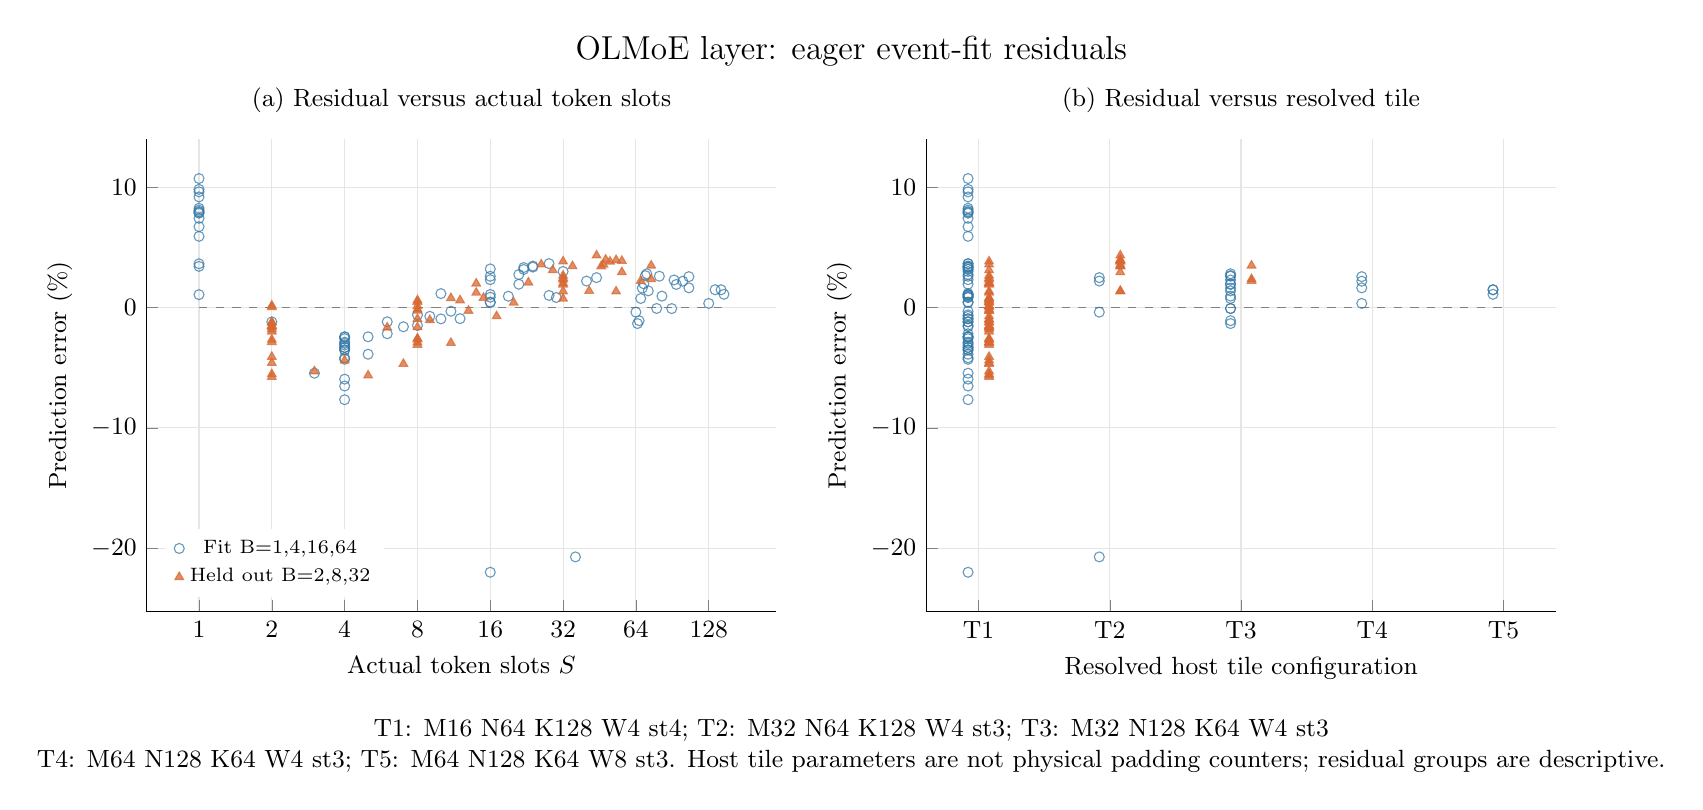
\begin{tikzpicture}
\definecolor{cal}{HTML}{3478A5}\definecolor{test}{HTML}{D76832}\definecolor{profile}{HTML}{3B8A5A}
\begin{groupplot}[group style={group size=2 by 1,horizontal sep=1.9cm},width=8.0cm,height=6.0cm,scale only axis,axis lines*=left,grid=major,grid style={gray!20},tick label style={font=\small},label style={font=\small},title style={font=\small},legend style={font=\scriptsize,draw=none},unbounded coords=jump]
\nextgroupplot[title={(a) Residual versus actual token slots},xlabel={Actual token slots $S$},ylabel={Prediction error (\%)},xmode=log,log basis x=2,xtick={1,2,4,8,16,32,64,128},xticklabels={1,2,4,8,16,32,64,128},legend pos=south west]\addplot[only marks,color=cal,mark=o,mark size=1.8pt,opacity=0.75] coordinates {(1,1.07645962773) (1,9.62477130164) (1,5.9239947836) (2,-1.18666590904) (1,3.64082308243) (1,8.10226307591) (3,-5.45433800069) (1,6.7256057143) (1,7.42483866818) (4,-4.29900425693) (1,7.97912639875) (1,9.1982615861) (5,-2.42909467686) (1,7.84651920017) (1,8.26169617597) (6,-2.17430981602) (1,9.83085088403) (1,10.7280331576) (7,-1.59517300671) (1,3.42590309956) (1,7.91400287206) (8,-1.48568124733) (4,-4.16767633238) (4,-7.65710832465) (5,-3.87824941202) (6,-1.18030598684) (4,-3.53174084381) (4,-2.44984049692) (8,-0.605467452606) (4,-2.58326898666) (4,-2.41853771955) (10,1.16327345806) (4,-3.32201783969) (4,-3.50302831472) (12,-0.919653654516) (4,-3.31549831848) (4,-6.52214195588) (9,-0.724376528077) (4,-2.97685731038) (4,-2.8782436283) (10,-0.939482192718) (4,-5.94909985523) (4,-3.1189923762) (11,-0.303315521845) (16,0.419473337706) (16,1.08994093422) (19,0.943901475471) (21,2.7445327204) (16,3.21600747053) (22,3.1714504738) (24,3.45218408425) (16,2.6044535547) (22,3.33118637069) (28,3.65618445956) (16,2.31963854739) (24,3.36553756272) (32,3.00363702401) (16,0.862694551349) (21,1.94304586758) (36,-20.7285437787) (16,-22.0044014751) (28,1.0083072566) (40,2.20517442905) (16,0.46304350917) (30,0.835519320158) (44,2.49140103934) (64,-0.380733434085) (65,-1.3278197505) (72,1.39138669945) (78,-0.0726222107891) (66,-1.08905355395) (80,2.60972628428) (90,-0.0833497135842) (67,0.754844447006) (82,0.952938115859) (106,1.64130993957) (68,1.61969110028) (92,2.2963404954) (128,0.344849697501) (69,1.97344872698) (94,1.9220080543) (144,1.48178978699) (70,2.65853245693) (100,2.193697175) (136,1.48439434081) (71,2.80948140702) (106,2.57158453645) (148,1.10519873754)};
\addlegendentry{Fit B=1,4,16,64}
\addplot[only marks,color=test,mark=triangle*,mark size=1.8pt,opacity=0.75] coordinates {(2,-5.53197706794) (2,0.166824700394) (2,-2.6644774709) (3,-5.29647080422) (2,-1.49989765971) (2,0.0403273656092) (4,-4.38756679863) (2,-2.85965316683) (2,-4.0942537898) (5,-5.6400819658) (2,-1.22315248976) (2,-1.23002511933) (6,-1.65628081622) (2,-1.8033122779) (2,-5.76300668243) (7,-4.67756988506) (2,-4.59543125784) (2,-1.62169695001) (8,-2.56545147106) (2,-1.9884221115) (2,-1.52197008167) (9,-1.03301600266) (8,-1.62673030044) (8,-0.942383078558) (8,-0.14437019241) (11,0.78914103219) (8,0.133330892906) (8,0.605893253647) (14,2.00262785623) (8,-2.8861629439) (11,-2.93564887862) (17,-0.715575327312) (8,-3.08952080026) (12,0.604181624382) (20,0.410835726286) (8,-2.63777852827) (13,-0.2612260876) (23,2.08832217693) (8,0.48689828352) (14,1.23901858416) (26,3.58617861352) (8,-0.254942115498) (15,0.807299989513) (29,3.11427548481) (32,3.84032853963) (32,2.33116070014) (41,1.3932938774) (35,3.44734587365) (32,1.91426102191) (46,3.43994742507) (48,3.9870936499) (32,2.03318029498) (50,3.82821389719) (53,3.95159096834) (32,2.46311335255) (56,3.88508396092) (44,4.33552169581) (32,2.65670497586) (47,3.57053254768) (67,2.22443884616) (32,1.35814392501) (56,2.94494960437) (74,3.49488945166) (32,0.73962474072) (74,2.36755476911) (53,1.34375729433)};
\addlegendentry{Held out B=2,8,32}\addplot[gray,dashed,forget plot,domain=1:148] {0};
\nextgroupplot[title={(b) Residual versus resolved tile},xlabel={Resolved host tile configuration},ylabel={Prediction error (\%)},xtick={1,2,3,4,5},xticklabels={T1,T2,T3,T4,T5},xmin=0.6,xmax=5.4]\addplot[only marks,color=cal,mark=o,mark size=1.8pt,opacity=0.75] coordinates {(0.92,1.07645962773) (0.92,9.62477130164) (0.92,5.9239947836) (0.92,-1.18666590904) (0.92,3.64082308243) (0.92,8.10226307591) (0.92,-5.45433800069) (0.92,6.7256057143) (0.92,7.42483866818) (0.92,-4.29900425693) (0.92,7.97912639875) (0.92,9.1982615861) (0.92,-2.42909467686) (0.92,7.84651920017) (0.92,8.26169617597) (0.92,-2.17430981602) (0.92,9.83085088403) (0.92,10.7280331576) (0.92,-1.59517300671) (0.92,3.42590309956) (0.92,7.91400287206) (0.92,-1.48568124733) (0.92,-4.16767633238) (0.92,-7.65710832465) (0.92,-3.87824941202) (0.92,-1.18030598684) (0.92,-3.53174084381) (0.92,-2.44984049692) (0.92,-0.605467452606) (0.92,-2.58326898666) (0.92,-2.41853771955) (0.92,1.16327345806) (0.92,-3.32201783969) (0.92,-3.50302831472) (0.92,-0.919653654516) (0.92,-3.31549831848) (0.92,-6.52214195588) (0.92,-0.724376528077) (0.92,-2.97685731038) (0.92,-2.8782436283) (0.92,-0.939482192718) (0.92,-5.94909985523) (0.92,-3.1189923762) (0.92,-0.303315521845) (0.92,0.419473337706) (0.92,1.08994093422) (0.92,0.943901475471) (0.92,2.7445327204) (0.92,3.21600747053) (0.92,3.1714504738) (0.92,3.45218408425) (0.92,2.6044535547) (0.92,3.33118637069) (0.92,3.65618445956) (0.92,2.31963854739) (0.92,3.36553756272) (0.92,3.00363702401) (0.92,0.862694551349) (0.92,1.94304586758) (1.92,-20.7285437787) (0.92,-22.0044014751) (0.92,1.0083072566) (1.92,2.20517442905) (0.92,0.46304350917) (0.92,0.835519320158) (1.92,2.49140103934) (1.92,-0.380733434085) (2.92,-1.3278197505) (2.92,1.39138669945) (2.92,-0.0726222107891) (2.92,-1.08905355395) (2.92,2.60972628428) (2.92,-0.0833497135842) (2.92,0.754844447006) (2.92,0.952938115859) (3.92,1.64130993957) (2.92,1.61969110028) (2.92,2.2963404954) (3.92,0.344849697501) (2.92,1.97344872698) (2.92,1.9220080543) (4.92,1.48178978699) (2.92,2.65853245693) (3.92,2.193697175) (4.92,1.48439434081) (2.92,2.80948140702) (3.92,2.57158453645) (4.92,1.10519873754)};
\addplot[only marks,color=test,mark=triangle*,mark size=1.8pt,opacity=0.75] coordinates {(1.08,-5.53197706794) (1.08,0.166824700394) (1.08,-2.6644774709) (1.08,-5.29647080422) (1.08,-1.49989765971) (1.08,0.0403273656092) (1.08,-4.38756679863) (1.08,-2.85965316683) (1.08,-4.0942537898) (1.08,-5.6400819658) (1.08,-1.22315248976) (1.08,-1.23002511933) (1.08,-1.65628081622) (1.08,-1.8033122779) (1.08,-5.76300668243) (1.08,-4.67756988506) (1.08,-4.59543125784) (1.08,-1.62169695001) (1.08,-2.56545147106) (1.08,-1.9884221115) (1.08,-1.52197008167) (1.08,-1.03301600266) (1.08,-1.62673030044) (1.08,-0.942383078558) (1.08,-0.14437019241) (1.08,0.78914103219) (1.08,0.133330892906) (1.08,0.605893253647) (1.08,2.00262785623) (1.08,-2.8861629439) (1.08,-2.93564887862) (1.08,-0.715575327312) (1.08,-3.08952080026) (1.08,0.604181624382) (1.08,0.410835726286) (1.08,-2.63777852827) (1.08,-0.2612260876) (1.08,2.08832217693) (1.08,0.48689828352) (1.08,1.23901858416) (1.08,3.58617861352) (1.08,-0.254942115498) (1.08,0.807299989513) (1.08,3.11427548481) (1.08,3.84032853963) (1.08,2.33116070014) (2.08,1.3932938774) (2.08,3.44734587365) (1.08,1.91426102191) (2.08,3.43994742507) (2.08,3.9870936499) (1.08,2.03318029498) (2.08,3.82821389719) (2.08,3.95159096834) (1.08,2.46311335255) (2.08,3.88508396092) (2.08,4.33552169581) (1.08,2.65670497586) (2.08,3.57053254768) (3.08,2.22443884616) (1.08,1.35814392501) (2.08,2.94494960437) (3.08,3.49488945166) (1.08,0.73962474072) (3.08,2.36755476911) (2.08,1.34375729433)};\addplot[gray,dashed,forget plot,domain=1:5] {0};
\end{groupplot}
\path (group c1r1.north west) -- node[above=0.8cm,font=\large] {OLMoE layer: eager event-fit residuals} (group c2r1.north east);
\path (group c1r1.south west) -- node[below=1.25cm,align=center,font=\small] {T1: M16 N64 K128 W4 st4; T2: M32 N64 K128 W4 st3; T3: M32 N128 K64 W4 st3\\T4: M64 N128 K64 W4 st3; T5: M64 N128 K64 W8 st3. Host tile parameters are not physical padding counters; residual groups are descriptive.} (group c2r1.south east);
\end{tikzpicture}\end{document}
